
\documentclass[a4paper,11pt]{article}

\usepackage[utf8]{inputenc}
\usepackage[T1]{fontenc}
\usepackage{verbatim}        % Wanted multiline comments
\usepackage{amsmath}         % Needed some math mode stuff
\usepackage{graphicx}        % Kinda useless, I just used it to display Borat
\usepackage{tikz}            % Pretty picturessss
\usetikzlibrary{positioning} % Mah nodes need GPS
\usetikzlibrary{calc}        % Whaaat ? Math in tikz ? Is this real life ?

\begin{document}

% ==================== title ====================
\title{Rapport de projet}
\author{Alexis Laouar, Rémi Oudin, Kévin Le Run}
\date{}
\maketitle
% ===============================================

\section{Vue d'ensemble}

L'architecture du moteur de jeu est une variante du Modèle-Vue-Contrôleur où les
modèles ne sont pas purs et ont une certaine part de contrôle.

% ==================== m-v-c figure ====================
\begin{figure}[h]
  \centering
  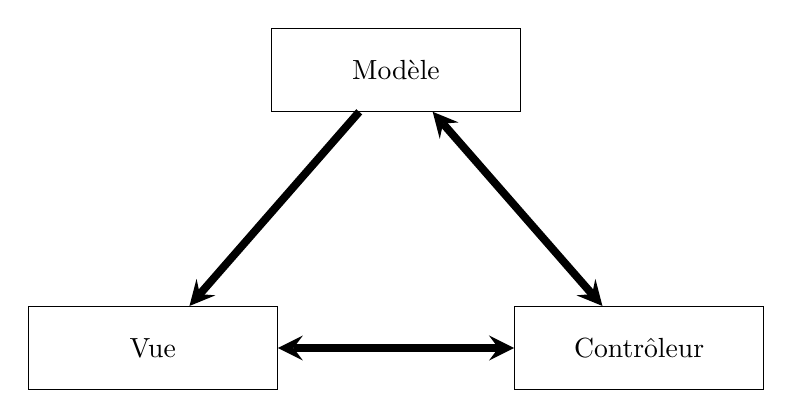
\begin{tikzpicture}[
      elementblock/.style={draw,rectangle,minimum height=3em, minimum width=9em},
      node distance=3cm]
    % Blocks
    \node[elementblock]                                     (view)      {Vue};
    \node[elementblock,right=of view]                       (controller){Contrôleur};
    \node[elementblock,above=of {$(view)!0.5!(controller)$}](model)     {Modèle};

    % Arrows
    \draw[         -{stealth},thick,line width=0.1cm] (model) edge (view);
    \draw[{stealth}-{stealth},thick,line width=0.1cm] (model) edge (controller) (controller) edge (view);

  \end{tikzpicture}
  \caption{Modèle-Vue-Contrôleur}
\end{figure}
% ======================================================

Les contrôleurs sont placés dans le package \texttt{runtime}, les modèles dans
le package \texttt{game\_mechanics} et les vues dans le package \texttt{gui}.

\section{Les contrôleurs}

Le contrôleur principal est l'objet \texttt{Controller}. Il contient la boucle
\texttt{update}-\texttt{render} ainsi que l'ensemble des modèles actifs :
les tours, les ennemis et les projectiles. À chaque tour de boucle, tous ces
modèles sont mis à jour et dessinés à l'écran. La mise à jour des mouvements se
fait par méthode d'Euler (plus de détails en section \ref{models}). \\

\noindent Le \texttt{SpawnScheduler} est un contr\^oleur qui g\`ere
l'apparition des ennemis. Il contient une file de paires
<temps,type d'ennemi> et fait appa\^itre l'ennemi du type correspondant quand
le temps est atteint.

% Needs more stuff in here :)

\section{Modèles} \label{models}

Pour les modèles, nous avons distingués 3 modèles principaux.

\subsection{Les ennemis}
Les ennemis, qui possèdent leur chemin et vont principalement avancer en
recalculant la trajectoire au fur et à mesure, à l'aide de la méthode d'Euler.
Les ennemis ont les attributs suivants:
\begin{itemize}
    \item \texttt{hp}, qui représente leurs points de vie
    \item \texttt{shield}, qui représente la réduction de dégâts
    \item \texttt{Speed}, qui représente leur vitesse de déplacement
    \item \texttt{Reward}, la récompense.
    \item \texttt{bunny\_type}, le type de l'ennemi
\end{itemize}

Le chemin d'un ennemi est constitu\'e d'un liste de points de passage.
\`A chaque mise \`a jour du jeu, l'ennemi effectue une interpolation lin\'eaire
entre le point de passage pr\'ec\'edent et le suivant. La distance qu'il
parcoure est d\'etermin\'ee par m\'ethode d'Euler:
$$ distance(t+\Delta t) = distance(t) + vitesse * \Delta t $$
À chaque mise à jour par le contrôleur, les monstres vérifient leur nombre de HP,
et demandent au contrôleur de l'oublier s'ils atteignent un nombre de HP négatif. \\

\noindent Afin de g\'erer plusieurs types d'ennemis, chaque instance d'ennemi poss\`ede un
objet type qui impl\'emente un trait de type.

\subsection{Les tours}

Une tour a une position fixe, et diverses caractéristiques, dont la portée, les
dégâts, le coût, et le cooldown. Pour tirer, la tour prend à chaque nouveau tir
l'ennemi qui est le plus avancé vers le core, et crée un objet projectile dont
la cible est le l'ennemi visé. Il transmet les propriétés de dégâts et de vitesse
du projectile à celui-ci. \\

\noindent De m\^eme que pour les ennemis, les tours poss\`edent un objet type
impl\'ementant un trait de type.

\subsection{Les projectiles}

Un projectile est un objet créé par une tour. Il a pour attributs:
\begin{itemize}
    \item une cible qui est un ennemi,
    \item une vitesse,
    \item une position courante,
    \item des dégâts.
\end{itemize}

Il suit son ennemi, c'est-à-dire qu'à chaque étape, il va récupérer la position
courante de sa cible, et se diriger vers lui. On considère que si après avoir bougé,
un projectile a dépassé sa cible, il l'a touché. Alors, le projectile demande à
sa cible de se retirer des HP.

\section{Vues}

Le panneau \texttt{MapPanel} dessine sur la fen\^etre le contenu de la carte du
jeu: tuiles, tours, ennemis, ... Il est redessin\'e a chaque tour de boucle. \\

\noindent Le panneau \texttt{InfoPanel} dessine sur la fen\^etre des informations g\'enerales
sur l'\'etat du jeu: or, vies restantes, num\'ero de vague, ... \\

\noindent Le panneau \texttt{TowerPanel} dessine sur la fen\^etre les informations sur
la tour actuellement s\'electionn\'ee si une tour est s\'electionn\'ee. \\

\noindent En plus de ces vues, divers boutons ont \'et\'e rajout\'es \`a
l'interface: bouton d'achat et de vente de tours, lancement de la vague, ...

\section{Autres fonctionnalités développées}

\subsection{Génération automatique de vagues}

\subsubsection*{Encodage des vagues}

Les vagues sont stockées dans des fichiers \texttt{.csv} de la forme suivante :

\begin{verbatim}
0.000000, Bunny
0.249445, Bunny
0.498891, HeavyBunny
0.748336, Bunny
0.997781, Hare
1.247226, Hare
1.496672, HeavyBunny
1.746117, Bunny
1.995562, Bunny
2.245007, Bunny
2.494453, Bunny
2.743898, HeavyBunny
2.993343, Bunny
3.242788, Bunny
...
\end{verbatim}

Le flottant est le temps (en secondes) d'apparition de l'unité, et le string qui suit est son identifiant. \newline

\subsubsection*{Génération des vagues}

Les fichiers de vagues sont générés automatiquement par un script \texttt{CamL} qui reçoit en argument le numéro de la vague. Chaque unité dispose des attributs suivants :

\begin{enumerate}
\item Son nom.
\item Sa difficulté, c'est-à-dire à quel point cette unité sera difficile à vaincre.
\item La première vague possible d'apparition.
\item Sa rareté, qui dépend du numéro de la vague. Par exemple, l'unité de base sera commune en début de jeu, puis sera progressivement remplacée par des unités plus difficiles.
\end{enumerate}

Etant donné un numéro de vague, le programme génère une vague aléatoire comme suit.

\begin{itemize}
\item A partir du numéro de la vague, un indice de difficulté est calculé selon une fonction donnée. Actuellement, il s'agit d'un polynôme de degré trois.
\item Encore à partir du numéro de la vague, un temps d'apparition $dt$ est calculé. Actuellement, ce temps décroît d'une seconde à un dixième de seconde avec une décroissance en $\frac{1}{x^{0.7}}$.
\item A partir des raretés des unités, une unité est choisie aléatoirement pour apparaître à l'instant présent. On compare ensuite sa difficulté à la difficulté de la vague : soit $d = \text{diff}_{\text{vague}} - \text{diff}_{\text{unité}}$.
  \begin{itemize}
  \item Si $d >= 0$, l'unité peut apparaître ; on écrit donc dans le fichier de sortie l'instant présent ainsi que le nom de l'unité, et on recommence cet algorithme à partir d'une date incrémentée de $dt$.
  \item Si $d < 0$, l'unité est trop puissante pour apparaître. Si la difficulté est telle qu'une des unités peut apparaître, on recommence ; sinon, l'algorithme se termine.
  \end{itemize}
\end{itemize}

L'intérêt de cette méthode de génération est que l'utilisation de fonctions pour la difficulté d'une vague, la rareté d'une unité et le temps d'apparition des unités permet très facilement d'effectuer des modification d'équilibrage d'une part en ne modifiant que ces fonctions et non le programme, et d'autre part nous laisse une grande liberté d'action sur l'allure des vagues tout au long du jeu.

\begin{comment}

  \section{Conclusion} % Maybe ?

  Ca marche. \newline
  \begin{figure}[h]
    
\includegraphics{great_success.png} 
  \end{figure}

\end{comment}



% TODO

\end{document}
